\subsection{Design Constraints}

\subsubsection{Software Constraints}
\begin{enumerate}
	\item Device Accelerometer Support:
	\newline
	Given that a device does has an accelerometer, the device manufacturer must provide a software interface to interact with the device's accelerometer.
\end{enumerate}

\subsubsection{Hardware Constraints}
\begin{enumerate}
	\item Accelerometer:
	\newline
	Not all devices models are made equal. Some older devices do not have accelerometers to track steps with. The accuracy of accelerometers also vary from different device manufacturers.
	\item Battery Life:
	\newline
	To track steps continuously with a background process will greatly impact the battery life of devices with small battery capacities. 
\end{enumerate}

\subsection{Software System Attributes} 
\subsubsection{Reliability} 
The fitness module must be able to accurately and reliably track movement through the devices accelerometer. This accuracy and reliability ensures that the calculation of steps, calories and other health related data is accurate. The accuracy and reliability requirements are to ensure that milestones and awards are distributed accurately.    

\subsubsection{Efficiency} 
In order for the application to efficiently count steps and calculate other health metrics, the fitness module needs efficient algorithms to calculate the steps and other health metrics quickly from the data it recives from the accelerometer.  

\subsubsection{Portability} 
The fitness module should be able to work on both iOS and Android devices. There should also be no discernible differences between the fitness module on iOS and the fitness module on Android devices. They should also yield the same the same health metrics. 

\subsubsection{Coupling} 
The fitness module should also integrate with the user module. It should be able to request the users age and name. The fitness module should also be able to write data such as the users height and weight. Minimal helth metrics should also be sent to the user module to be stored on the server. 


\subsection{Activity Diagram}
See figure~\ref{fig:fitness_activity_diagram} on page~\pageref{fig:fitness_activity_diagram}
\begin{figure}
	\centering
	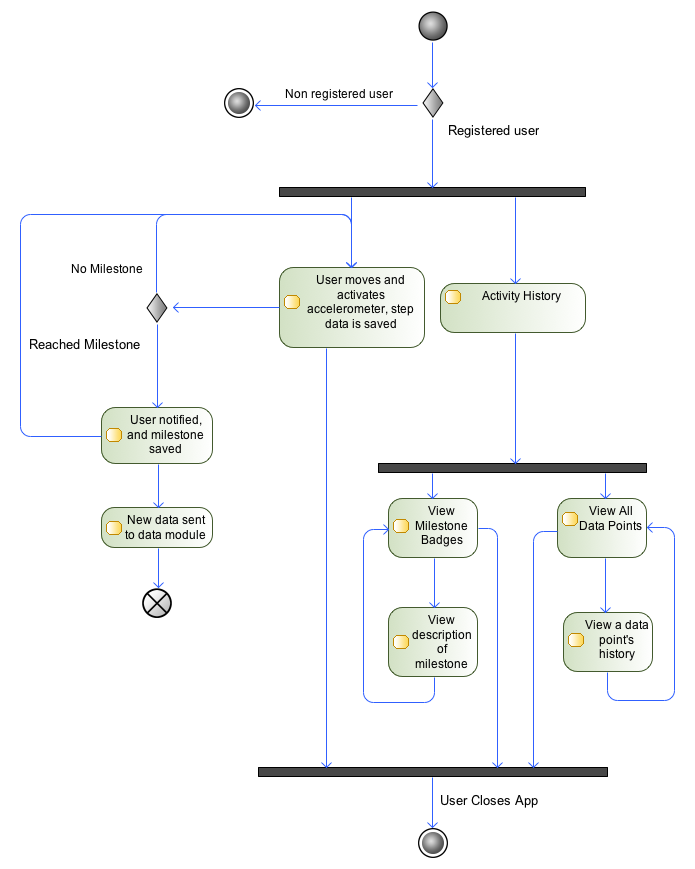
\includegraphics[scale=0.54]{Fitness/fitness_activity_diagram.png}
	\caption{Fitness Activity Diagram}
	\label{fig:fitness_activity_diagram}
\end{figure}

\subsection{State Diagrams}
See figure~\ref{fig:fitness_state_diagram} on page~\pageref{fig:fitness_state_diagram}
\begin{figure}
	\centering
	\includegraphics[scale=0.54]{Fitness/fitness_state_diagram.png}
	\caption{Fitness State Diagram}
	\label{fig:fitness_state_diagram}
\end{figure}

\subsection{Deployment Diagram}
See figure~\ref{fig:fitness_deployment_diagram} on page~\pageref{fig:fitness_deployment_diagram}
\begin{figure}
	\centering
	\includegraphics[scale=0.54]{Fitness/fitness_deployment_diagram.png}
	\caption{Fitness Deployment Diagram}
	\label{fig:fitness_deployment_diagram}
\end{figure}